\begin{frame}
\frametitle{NEXT2-BOLD}

\begin{figure}[tbh!]
  \begin{center}
      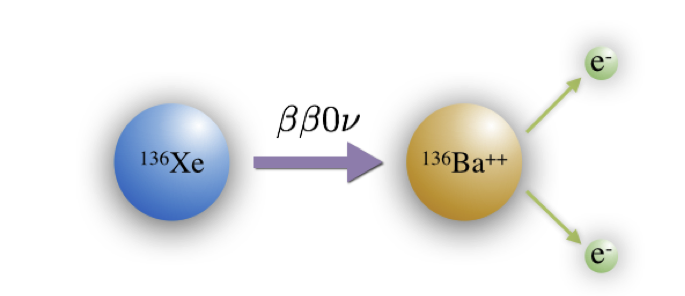
\includegraphics[width=0.75\textwidth]{moriond/bata.png}   
  \end{center}
\end{figure}
\begin{itemize} 
\item If the \Bapp\ produced in the $\XE \rightarrow \Bapp + 2 e (+ 2  \nu)$ can be detected efficiently, one could aim for the {\bf BOLD} (Barium iOn Light Detection) option.  
\item Detecting ``tagging'' the \Bapp\ signaling a \bbonu\ process has been a long sought holy grail of xenon chambers. 
\item Dave Nygren's proposal to do it using SMFI (Single Molecule Fluorescence Imaging) could turn fantasy into reality.   
\end{itemize}
\end{frame}

\begin{frame}
\frametitle{A bright idea}
  \begin{center}
      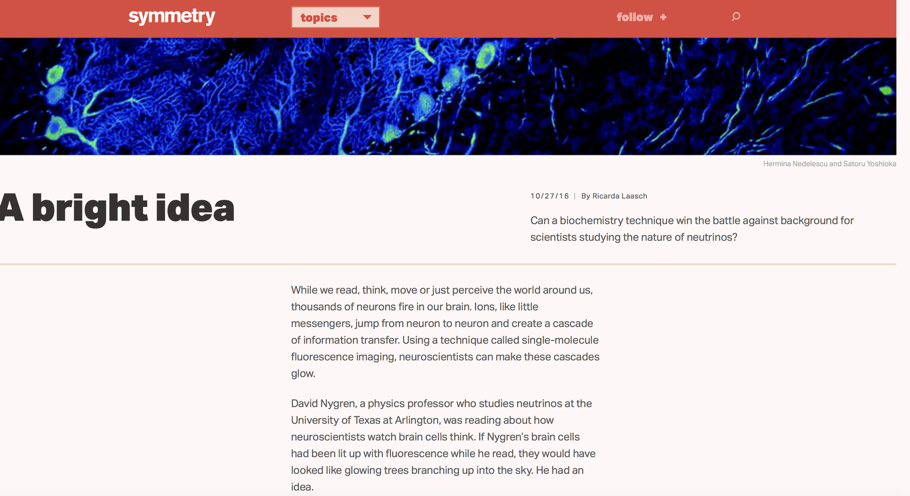
\includegraphics[width=0.75\textwidth]{moriond/nygren-smfi.png}   
  \end{center}
\begin{itemize} 
\item Dave Nygren's, 2016: \url{https://www.symmetrymagazine.org/article/a-bright-idea}    
\end{itemize}
\end{frame}

\begin{frame}
\frametitle{Single Molecule Fluorescence Imaging}
  \begin{center}
      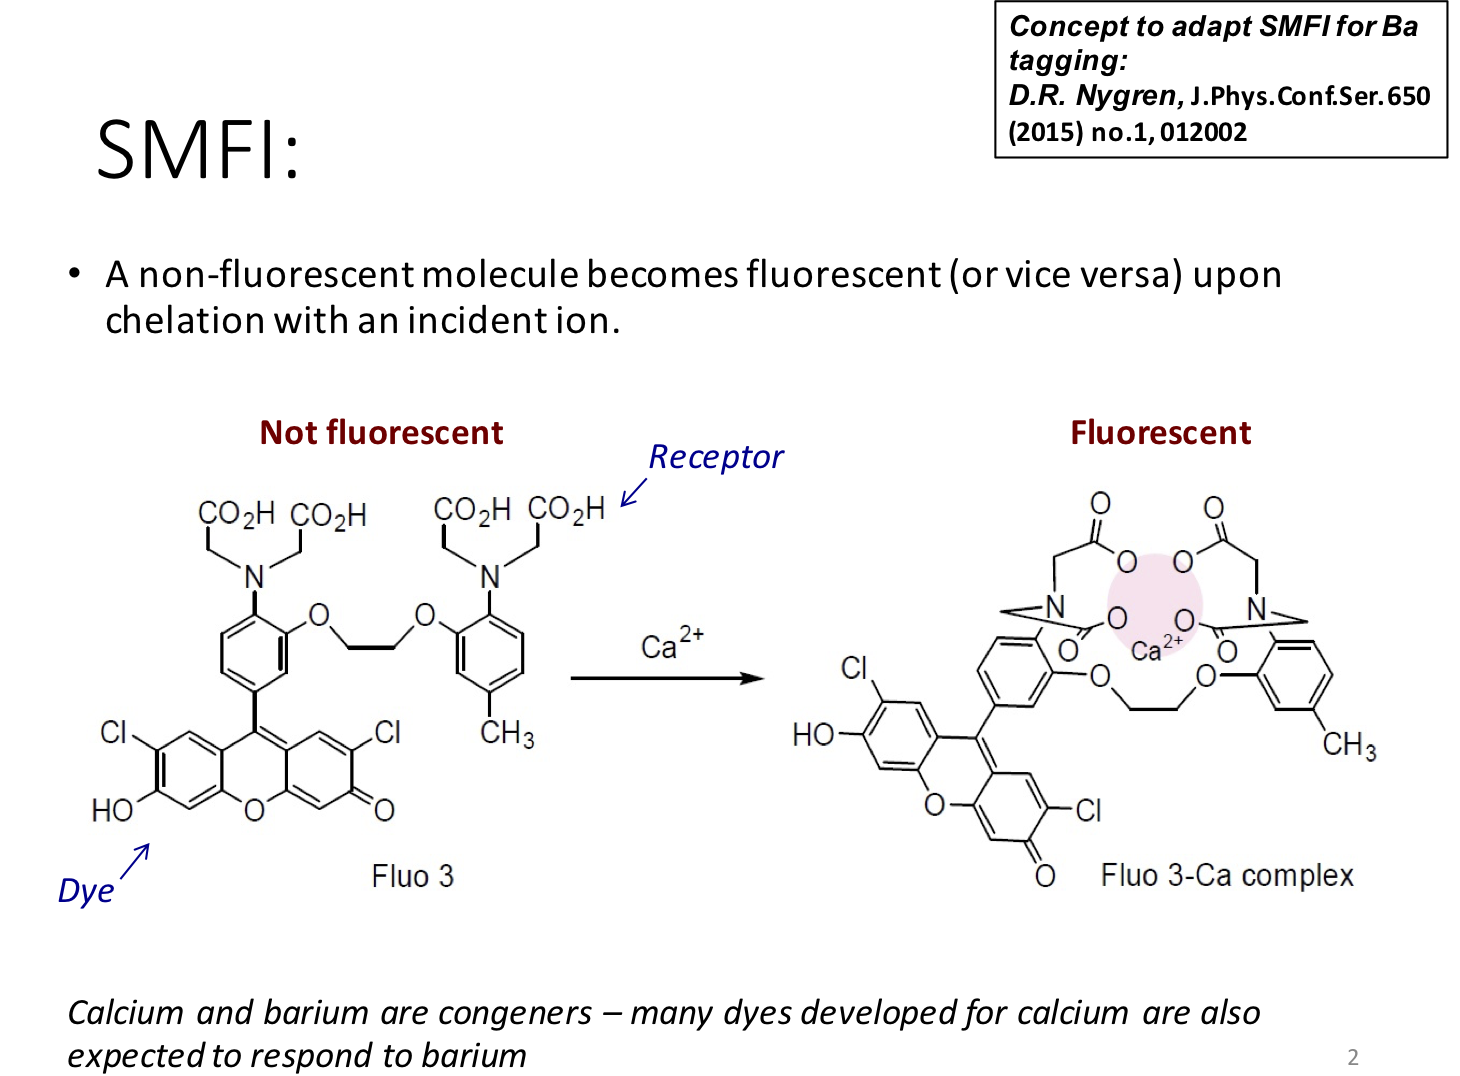
\includegraphics[width=0.75\textwidth]{moriond/smfi-concept.png}   
  \end{center}
\end{frame}

\begin{frame}
\frametitle{SMFI with \Bapp. Proof of concept}
  \begin{center}
      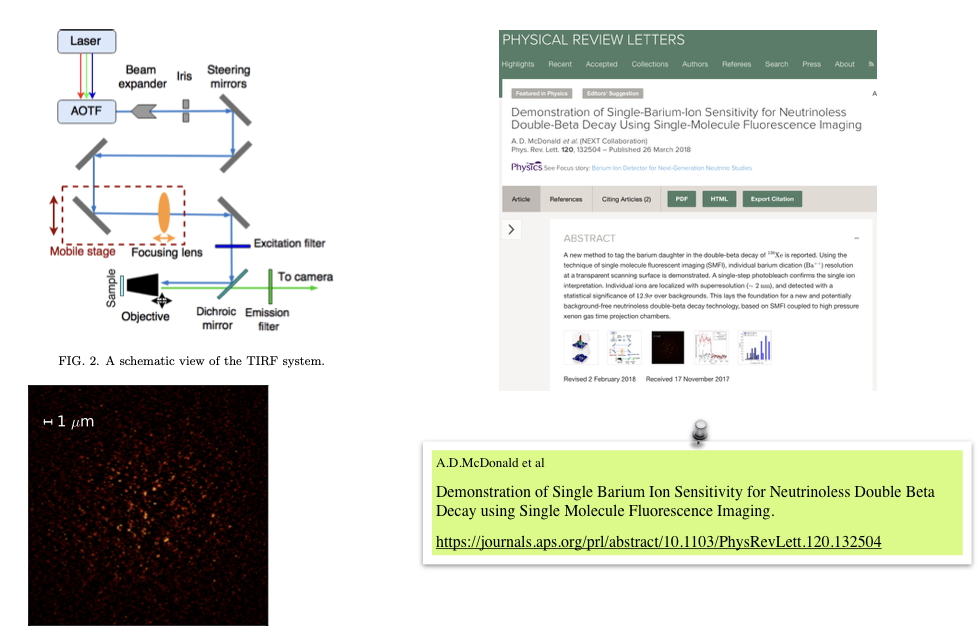
\includegraphics[width=0.85\textwidth]{moriond/sabat-poc.png}   
  \end{center}
\end{frame}

\begin{frame}
\frametitle{SMFI setup}
  \begin{center}
      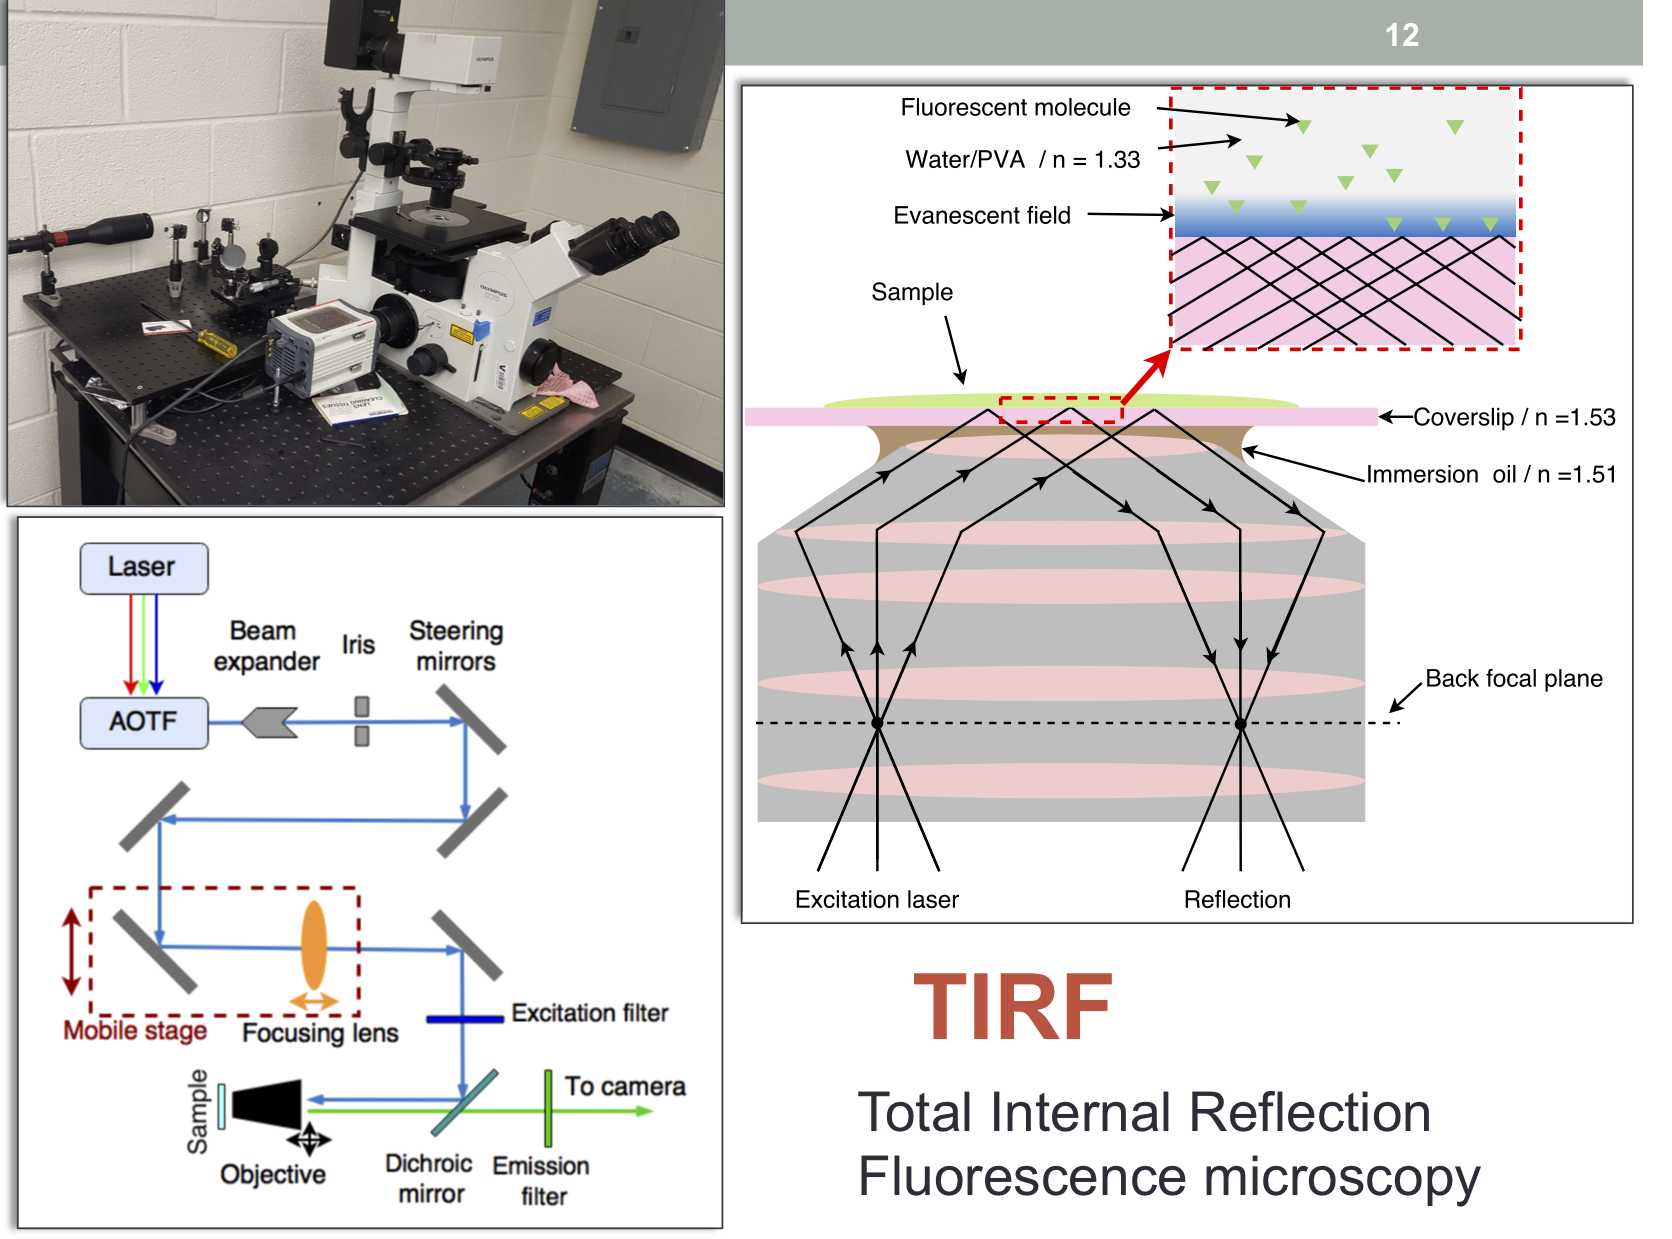
\includegraphics[width=0.85\textwidth]{moriond/smfi-setup.png}   
  \end{center}
\end{frame}


\begin{frame}
\frametitle{We see single molecules chelated with \Bapp!}
  \begin{center}
      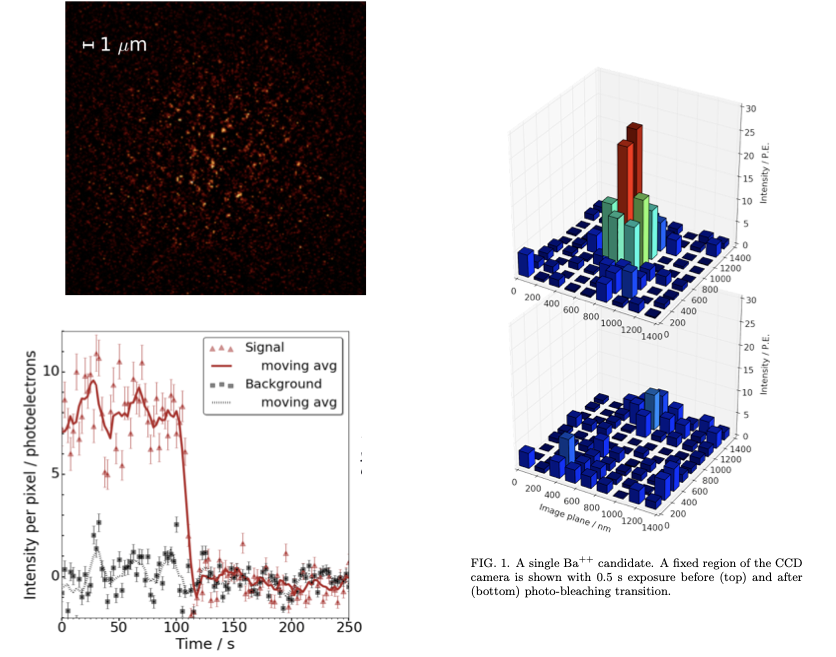
\includegraphics[width=0.85\textwidth]{moriond/smfi-observed.png}   
  \end{center}
\end{frame}



\begin{frame}
\frametitle{Next step? RITA}

\begin{columns}
 
\column{0.5\textwidth}
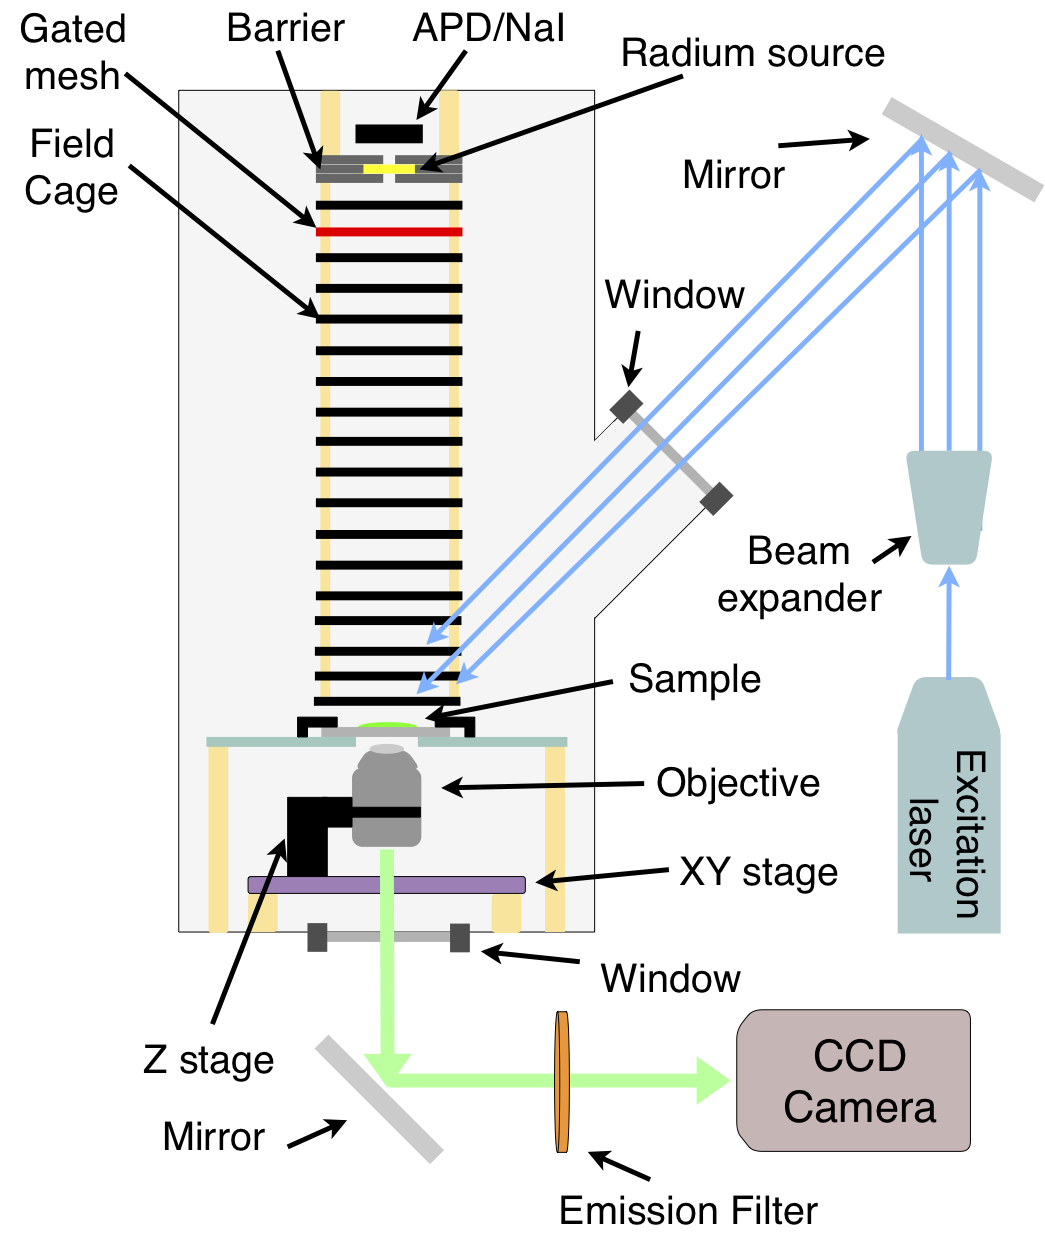
\includegraphics[scale=0.35]{moriond/rita.png}
 
\column{0.5\textwidth}

%\begin{figure}[tbh!]
%  \begin{center}
%      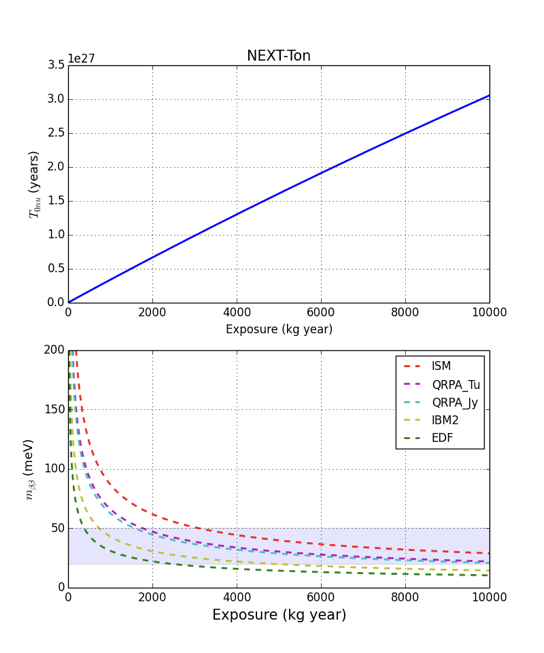
\includegraphics[width=0.4\textwidth]{moriond/next2-hd-sensi.png}
%   
%  \end{center}
% \end{figure}
 
\begin{itemize} 
\item RadIum TAgging (RITA) in dry medium (we can use several noble gases at different pressures).   
\item \Rapp\ produced by TH-228 decays. Radium and Barium are chemical "twin brothers" (same ionization potential, same radius, etc.). We can tag the production of \Rapp\ ions counting the recoiling alphas. 
\item Target will be a mon-layer of suitable molecules capable to capture the ion in gas and produce a strong fluorescence.
\item If RITA succeeds we may have a serious case for a BOLD NEXT-2.0 detector. 
\end{itemize}
\end{columns}
\end{frame}






